\section{Experimental Design}

\paragraph{Techniques to Evaluate Performance}
\begin{itemize}
\item Three main techniques
  \begin{itemize}
  \item Analytical Modeling
  \item Simulation
  \item Experimentation
  \end{itemize}
\end{itemize}


\paragraph{Analytical Modeling}
\begin{itemize}
\item Get intuition about system performance
  \begin{itemize}
  \item Without actually implementing it!
  \end{itemize}

\item Simple model for virtual memory system with paging:

  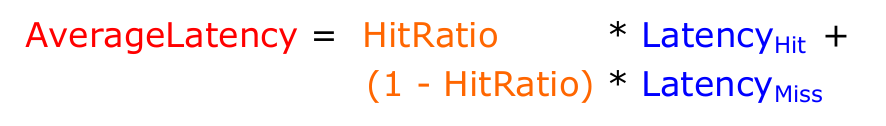
\includegraphics[scale=0.15]{graphics/model-virtual-memory.png}

\item With high hit ratio (say, >95\%), average time can be
  pretty close to main memory
  \begin{itemize}
  \item Some requests still require going to disk, of course, and
    take full disk latency blow
  \end{itemize}

\item How can we know the hit ratio?
\end{itemize}


\paragraph{Simulation}
\begin{itemize}
\item Study properties of hard-to-model process, e.g.,
  locality of workloads vs. hit ratio in cache
\item Configure model with known parameters
  \begin{itemize}
  \item In our example,
    {\color{blue} $\text{Latency}_{\text{Hit}}$} and
    {\color{blue} $\text{Latency}_{\text{Miss}}$}
  \end{itemize}

\item Simulate behavior of system to get {\color{orange} HitRatio}
\end{itemize}


\paragraph{Simulation}

\begin{itemize}
\item {\color{green} Pros}
  \begin{itemize}
  \item Effort may be smaller than full-blown implementation
  \item Allows you to simulate ``impossible'' or
    hard-to-experiment-with scenarios → 10Ks of machines,
    next-generation flash disk not on the market yet
  \end{itemize}
\end{itemize}

\begin{itemize}
\item {\color{red} Cons}
  \begin{itemize}
  \item Estimating parameters
  \item Validating models and approximations
  \item Choosing workloads
  \end{itemize}
\end{itemize}


\paragraph{Choosing Workloads \& Datasets}
\begin{itemize}
\item Synthetic workloads \& datasets
  \begin{itemize}
  \item Example: use Zipf distribution to generate workload
    of page accesses (Zipf distribution: most frequent word occurs
    twice as often as 2. most frequent and 3 times as often as 3. most
    frequent etc.)
  \end{itemize}

\item Real workloads \& datasets
  \begin{itemize}
  \item Example: Take \textbf{trace} of page requests from
    real application
  \item replay trace on your simulator
  \end{itemize}

\item Combinations also possible
  \begin{itemize}
  \item Use real dataset but generate accesses using a distribution
  \end{itemize}

\item Issue: How can you tell if workload is representative?
\end{itemize}


\paragraph{Experimentation}
\begin{itemize}
\item \textbf{Implement} real system (or prototype)
\item \textbf{Measure} how it behaves with experiments
  \begin{itemize}
  \item most respected method
  \item but also requires most effort
  \end{itemize}

\item \textbf{Profile} system to determine where time goes
\end{itemize}

\paragraph{Simple Factor Experimentation}
\begin{itemize}
\item Understanding multiple influences
\item Vary one factor at a time, keep others fixed

\item Example: Skew of workload and size of cache
  \begin{itemize}
  \item Skew = 0.5, vary cache size from 1MB to 1GB
  \item Cache size = 500MB, vary skew from 0 to 1
  \end{itemize}

\item Care required:
  Parameters may \textbf{influence} each other!
\end{itemize}

\paragraph{Benchmarking}

\begin{itemize}
\item \textbf{Micro-benchmarks}
  \begin{itemize}
  \item Measure a specific variable or piece of code, e.g.,
    memory and disk latencies in small experiment to
    calibrate simulation model
  \end{itemize}

\item \textbf{Application-level benchmark}
  \begin{itemize}
  \item whole application designed to stress certain types of systems
  \item \textbf{SPEC} benchmarks for compute-intensive apps,
    web servers, file systems, and many others
  \item \textbf{TPC} benchmarks for databases
  \end{itemize}
\end{itemize}

\paragraph{Necessary Care with Executing Experiments}
\begin{itemize}
\item Select \textbf{event counts}
  \begin{itemize}
  \item Number of pages/chunks read
  \item Number of clock cycles elapsed → wall-clock time
  \end{itemize}

\item But control for \textbf{overhead} of event counting
  itself!

\item \textbf{Sampling / monitoring}
  \begin{itemize}
  \item e.g., I/O via iostat/vmstat
  \end{itemize}

\item ``\textbf{Statistics} can prove anything?!''
  \begin{itemize}
  \item Number of measurements
  \item Mean and variance
  \item confidence intervals
  \item dealing with outliers
  \item Setup matters!
  \end{itemize}
\end{itemize}


\paragraph{Comparing Alternatives}
\begin{itemize}
\item Two systems, with throughput-oriented
  measurements $R_2$ and $R_1$
  \begin{itemize}
  \item Both systems travel same distance $D$, i.e., do same
    work but take different time
  \item $R_2 = D / T_2$; $R_1 = D /T_1$
  \end{itemize}


\item Speedup
  \begin{itemize}
  \item $S_{2,1} = R_2 / R_1 = T_1 / T_2$
  \end{itemize}

\item Relative change
  \begin{itemize}
  \item $\Delta_{2,1} = (R_2 - R_1) / R_1 = S_{2,1} - 1$
  \end{itemize}

\item Example statements
  \begin{itemize}
  \item System 2 is 1.4 times faster than System 1
  \item System 2 is 40\% faster than System 1
  \end{itemize}
\end{itemize}

\paragraph{Implementing All-or-Nothing Atomicity}
\begin{itemize}
\item Atomicity
  \begin{itemize}
  \item Transactions may abort (``Rollback'')
  \end{itemize}

\item Durability
  \begin{itemize}
  \item What if system stops running? (Causes?)
  \end{itemize}
\end{itemize}

\begin{minipage}{0.2\textwidth}
  \begin{itemize}
  \item Desired behavior after system restart
    \begin{itemize}
    \item {\color{blue} T1, T2, T3} should be
      {\color{blue} durable}
    \item {\color{red} T4, T5} should be {\color{red} aborted} \\
      (effects not seen)
    \end{itemize}
  \end{itemize}
\end{minipage}%
\begin{minipage}{0.2\textwidth}
  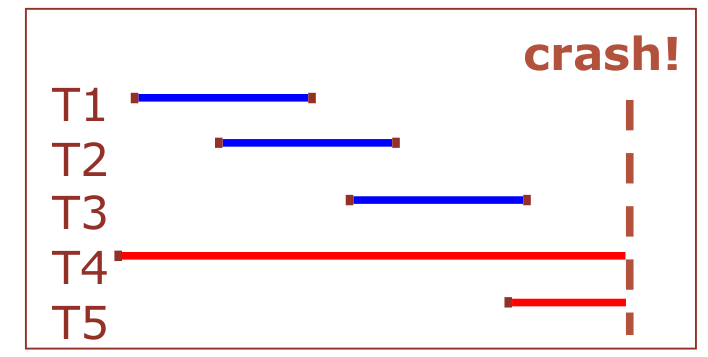
\includegraphics[scale=0.1]{graphics/crash.png}
\end{minipage}

\paragraph{Assumptions}
\begin{itemize}
\item Concurrency control is in effect
  \begin{itemize}
  \item Strict 2PL, in particular
  \end{itemize}

\item Updates are happening ``in place''
  \begin{itemize}
  \item i.e. data is overwritten on (deleted from) memory
    using READ / WRITE interface
  \item we will use two-level memory with buffer and disk
  \end{itemize}

\item Types of failures
  \begin{itemize}
  \item Crash
  \item Media failure
  \end{itemize}

\item Always fail-stop! (components notify that they have crashed)
\end{itemize}


\paragraph{Volatile vs. Nonvolatile vs.Stable Storage}
\begin{itemize}
\item Volatile Storage
  \begin{itemize}
  \item Lost in the event of a crash
  \item Example: main memory
  \end{itemize}

\item Nonvolatile Storage
  \begin{itemize}
  \item Not lost on crash, but lost on media failure
  \end{itemize}

\item Stable Storage
  \begin{itemize}
  \item Never lost
  \item How do you implement this one? (Replication only lower chance
    of failure)
  \end{itemize}
\end{itemize}

\paragraph{Surviving Crashes: How to handle the Buffer Pool?}


\begin{minipage}{0.2\textwidth}
  \begin{itemize}
  \item \textbf{Force} every write to disk?
    \begin{itemize}
    \item Poor response time
    \item But provides durability
    \end{itemize}

  \item \textbf{Steal} buffer-pool frames from uncommitted Xacts?
    \begin{itemize}
    \item If not, poor throughput
    \item If so, how can we ensure atomicity?
    \end{itemize}
  \end{itemize}
\end{minipage}%
\begin{minipage}{0.2\textwidth}
  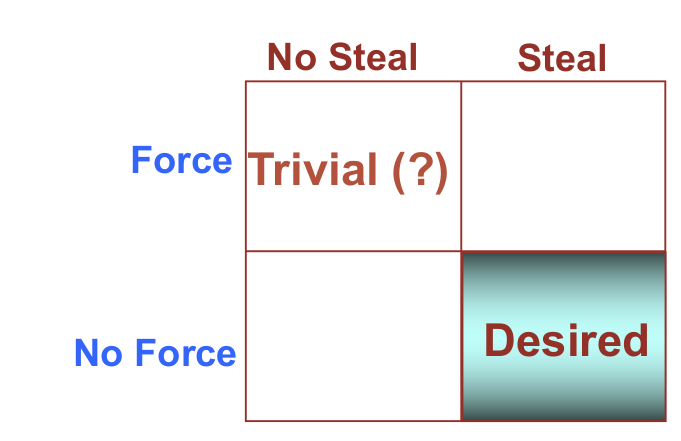
\includegraphics[scale=0.1]{graphics/force-steal.png}
\end{minipage}


\paragraph{More on Steal and Force}
\begin{itemize}
\item \textbf{STEAL} (why enforcing Atomicity is hard)
  \begin{itemize}
  \item to steal a frame F: current page in F (say P) is written to
    disk; some Xact holds a lock on P
    \begin{itemize}
    \item What if the Xact with the lock on P aborts?
    \item Must remember the old value of P at steal time
      (to support UNDOing the write to page P)
    \end{itemize}
  \end{itemize}

\item \textbf{NO FORCE} (why enforcing Durability is hard)
  \begin{itemize}
  \item What if system crashes before a modified page is written
    to disk?
  \item Write as little as possible, in a convenient place,
    at commit time, to support REDOing modifications
  \end{itemize}
\end{itemize}

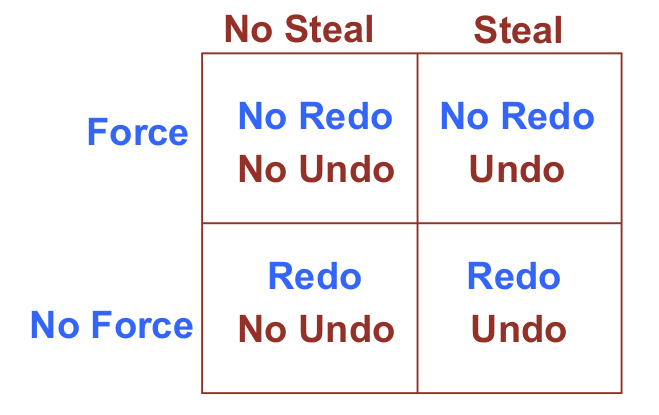
\includegraphics[scale=0.15]{graphics/force-steal-matrix.png}


\paragraph{Basic Idea: Logging}
\begin{itemize}
\item Record REDO and UNDO information, for every update, in a
  \textbf{log}
  \begin{itemize}
  \item Sequential writes to log (put it on a separate disk)
  \item Minimal info (diff) written to log, so multiple updates
    fit in a single log page
  \end{itemize}

\item \textbf{Log:} an ordered list of REDO/UNDO actions
  \begin{itemize}
  \item logical vs. physical logging
  \item example physical log record contains:

    {\color{blue} <XID, pageID, offset, length, old data, new data>}

  \item good compromise is physiological logging
  \end{itemize}
\end{itemize}

\paragraph{Write-Ahead Logging (WAL)}
\begin{itemize}
\item Golden Rule: Never modify the only copy!
\item The {\color{blue} Write-Ahead Logging} Protocol:
  \begin{enumerate}
  \item Must force the log record for an update \textbf{before} the
    corresponding data page gets to disk
  \item Must write all log records for a Xact \textbf{before commit}
  \end{enumerate}
\item \#1 guarantees Atomicity
\item \#2 guarantees Durability
\end{itemize}

\paragraph{Recovery Equations}

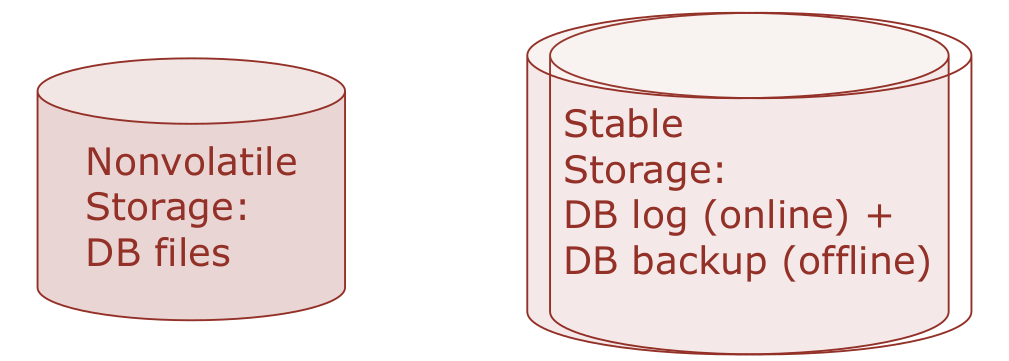
\includegraphics[scale=0.15]{graphics/recovery-eq.png}

\begin{itemize}
\item Crash Recovery: volatile memory lost
  \begin{itemize}
  \item Current DB = DB files + DB log
    ({\color{red} Since last transaction that did not complete}
  \end{itemize}

\item Media Recovery: nonvolatile storage lost
  \begin{itemize}
  \item Current DB = DB backup + DB log
    {\color{red} Since last checkpoint}
  \end{itemize}
\end{itemize}

% LocalWords:  HitRatio Datasets datasets Zipf dataset Benchmarking
% LocalWords:  latencies TPC iostat vmstat Atomicity Xacts atomicity
% LocalWords:  Xact UNDOing REDOing XID pageID WAL
